\documentclass[12pt, oneside]{book}

\usepackage{import}
\usepackage{../Packages/baupreamble}


\begin{document}


\chapter*{Appendices}
\appendix
%%=================================================
%%++++++++++++ Start writing here +++++++++++++++++
%%=================================================



% Please add the following required packages to your document preamble:
% \usepackage{booktabs}
	\captionof{Appendix}{Effect of interaction of arbuscular mycorrhizal fungi (AMF) and zinc fertilizer management on growth characters of hybrid maize Kohinoor 1820 \label{tableA1}}
	\begin{tabular*}{\textwidth}{@{}p{5.45cm}@{\extracolsep{\fill}}p{3.0cm}@{\extracolsep{\fill}}p{2.5cm}@{\extracolsep{\fill}}p{2.5cm}@{}}
		\toprule
		Combination             & Plant height\par (cm) & No. of leaves plant$^{-1}$ & Cob length\par (cm) \\ \midrule
		AMF0 × NoZinc           & 175.26 ± 9.3 b        & 11.07 ± 0.22            & 16.07 ± 0.73      \\
		AMF0 × Basal100         & 172.37 ± 3.8 b        & 11.75 ± 0.39            & 15.83 ± 1.34      \\
		AMF0 × Foliar100@EV     & 165.50 ± 8.04 c        & 10.68 ± 1.01            & 18.75 ± 2.49      \\
		AMF0 × Folar100@Rp      & 161.37 ± 14.8 d     & 12.11 ± 0.63            & 16.25 ± 1.84      \\
		AMF0 × Foliar@50EV+50Rp & 162.31 ± 4.53 d       & 11.57 ± 0.2             & 18.35 ± 0.99      \\
		AMF1 × NoZinc           & 165.03 ± 3.42 c       & 11.25 ± 0.3             & 16.40 ± 1.07       \\
		AMF1 × Basal100         & 175.88 ± 4.89 b       & 12.78 ± 0.75            & 16.94 ± 1.85      \\
		AMF1 × Foliar100@EV     & 184.36 ± 11.6 a       & 12.21 ± 0.21            & 17.49 ± 2.17      \\
		AMF1 × Folar100@Rp      & 173.64 ± 6.1 b        & 11.47 ± 0.87            & 16.72 ± 1.72      \\
		AMF1 × Foliar@50EV+50Rp & 164.10 ± 8.5 c         & 11.95 ± 0.91            & 19.94 ± 0.31      \\ \midrule
		p-value                   &   0.025                     & 0.840                      &   0.131 \\ \bottomrule
	\end{tabular*}
\begin{tablenotes}
\item[] Values and mean $\pm$ standard deviation; values in a column with different letters differ significantly at P = 0.05;
\item[]AMF0 = AMF non-inoculated, and AMF1 = AMF inoculated; NoZinc = no Zn fertilizer (control); Basal100 = 100\% recommended dose  (RD) of Zn added during final land preparation; Foliar100@EV = 100\% RD of Zn was applied as foliar spray (0.1\% ZnSO$_4$)  during early vegetative (EV) stage;  Folar100@Rp = 100\% RD of Zn fertilizer was applied as foliar spray during early reporductive (Rp) stage; Foliar@50EV+50Rp =  100\% RD of Zn was applied as foliar spray by equal split during  EV and Rp stages.
\end{tablenotes}


\newpage


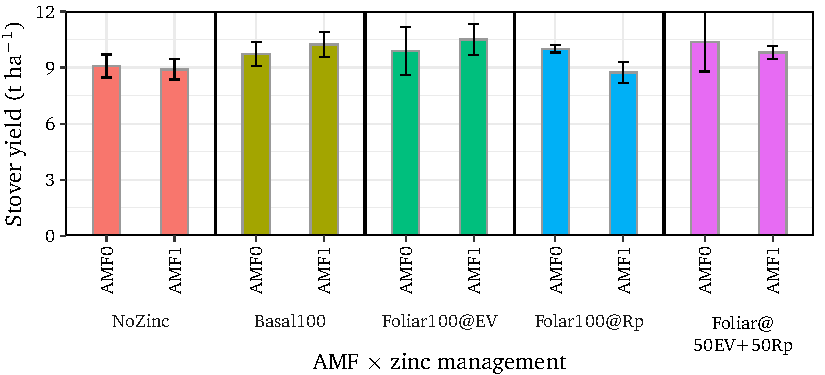
\includegraphics[width=\textwidth]{figures/figA2.pdf}
\captionof{Appendix}[Effects of interaction of AMF inoculation and Zn management on grain yield of hybrid maize Kohinoor 1820. AMF0 and AMF1 denote AMF inoculated and AMF non-inoculated]{Effects of interaction of AMF inoculation and Zn management on grain yield of hybrid maize Kohinoor 1820. AMF0 and AMF1 denote AMF inoculated and AMF non-inoculated, repsectively. NoZinc = no Zn fertilizer (control); Basal100 = 100\% recommended dose (RD) of Zn added during final land preparation; Foliar100@EV = 100\% RD of Zn was applied as foliar spray (0.1\% ZnSO4) during early vegetative (EV) stage; Folar100@Rp = 100\% RD of Zn fertilizer was applied as foliar spray during early reporductive (Rp) stage; Foliar@50EV+50Rp = 100\% RD of Zn was applied as foliar spray by equal split during EV and Rp stages. Vertical bar represents mean ± standard deviation; values of bars with different letters are significantly different at P=0.05} % caption can be placed on top of figure by putting it before \includegraphics command. Text inside [] will be shown in the list of appendices
\label{figA2}





%%=================================================
%%=================================================
\end{document}